%%%%%%%%%%%%%%%%%%%%%%%%%%%%%%%%%%%%%%%%%%%%%%%%%%%%%%%%%%%%%%%%%%%%%%%%%%%%%%%%%%%%%%%%%%%%%%%%%%%%%%%%%%%
%%%%%%%%%%%%%%%%%%%%%%%%%%%%%%%%%%%%%%%%%%%%%%%%%%%%%%%%%%%%%%%%%%%%%%%%%%%%%%%%%%%%%%%%%%%%%%%%%%%%%%%%%%%
%                                           EXAMPLE CODE                                                  %
%%%%%%%%%%%%%%%%%%%%%%%%%%%%%%%%%%%%%%%%%%%%%%%%%%%%%%%%%%%%%%%%%%%%%%%%%%%%%%%%%%%%%%%%%%%%%%%%%%%%%%%%%%%
%%%%%%%%%%%%%%%%%%%%%%%%%%%%%%%%%%%%%%%%%%%%%%%%%%%%%%%%%%%%%%%%%%%%%%%%%%%%%%%%%%%%%%%%%%%%%%%%%%%%%%%%%%%

%%%%%%%%%%%%%%%%%%%%%%%%%%%%%%%%%%%%%%%%%%%%%%%%%%%%%%%%%%%%%%%%%%%%%%%%%%%%%%%%%%%%%%%%%%%%%%%%%%%%%%%%%%%
%                                           INCLUDE PDF                                                   %
%%%%%%%%%%%%%%%%%%%%%%%%%%%%%%%%%%%%%%%%%%%%%%%%%%%%%%%%%%%%%%%%%%%%%%%%%%%%%%%%%%%%%%%%%%%%%%%%%%%%%%%%%%%
% \includepdf[pages=-]{null.PDF}

%%%%%%%%%%%%%%%%%%%%%%%%%%%%%%%%%%%%%%%%%%%%%%%%%%%%%%%%%%%%%%%%%%%%%%%%%%%%%%%%%%%%%%%%%%%%%%%%%%%%%%%%%%%
%                                           SAMPLE IMAGE COMMAND                                          %
%%%%%%%%%%%%%%%%%%%%%%%%%%%%%%%%%%%%%%%%%%%%%%%%%%%%%%%%%%%%%%%%%%%%%%%%%%%%%%%%%%%%%%%%%%%%%%%%%%%%%%%%%%%
% \includegraphics[scale=0.15, center]{null.PNG}

%%%%%%%%%%%%%%%%%%%%%%%%%%%%%%%%%%%%%%%%%%%%%%%%%%%%%%%%%%%%%%%%%%%%%%%%%%%%%%%%%%%%%%%%%%%%%%%%%%%%%%%%%%%
%                                           SUB-QUESTION FORMS                                            %
%%%%%%%%%%%%%%%%%%%%%%%%%%%%%%%%%%%%%%%%%%%%%%%%%%%%%%%%%%%%%%%%%%%%%%%%%%%%%%%%%%%%%%%%%%%%%%%%%%%%%%%%%%%
% \begin{enumerate}[label=(\roman*)]
%
% \end{enumerate}

% \begin{enumerate}[label=(\alph*)]
%
% \end{enumerate}

%%%%%%%%%%%%%%%%%%%%%%%%%%%%%%%%%%%%%%%%%%%%%%%%%%%%%%%%%%%%%%%%%%%%%%%%%%%%%%%%%%%%%%%%%%%%%%%%%%%%%%%%%%%
%                                           SCIENTIFIC NOTATION                                           %
%%%%%%%%%%%%%%%%%%%%%%%%%%%%%%%%%%%%%%%%%%%%%%%%%%%%%%%%%%%%%%%%%%%%%%%%%%%%%%%%%%%%%%%%%%%%%%%%%%%%%%%%%%%
% Number only: \num{1e-10}
% Number with units: \SI{1e-10}{\meter\per\second}

%%%%%%%%%%%%%%%%%%%%%%%%%%%%%%%%%%%%%%%%%%%%%%%%%%%%%%%%%%%%%%%%%%%%%%%%%%%%%%%%%%%%%%%%%%%%%%%%%%%%%%%%%%%
%                                           SIGMA NOTATION                                                %
%%%%%%%%%%%%%%%%%%%%%%%%%%%%%%%%%%%%%%%%%%%%%%%%%%%%%%%%%%%%%%%%%%%%%%%%%%%%%%%%%%%%%%%%%%%%%%%%%%%%%%%%%%%
%   Sum $\sum_{n=1}^{\infty} 2^{-n} = 1$ inside text
%
%   \[ \sum_{n=1}^{\infty} 2^{-n} = 1 \]

%%%%%%%%%%%%%%%%%%%%%%%%%%%%%%%%%%%%%%%%%%%%%%%%%%%%%%%%%%%%%%%%%%%%%%%%%%%%%%%%%%%%%%%%%%%%%%%%%%%%%%%%%%%
%                                           STANDARD MATRIX FORM                                          %
%%%%%%%%%%%%%%%%%%%%%%%%%%%%%%%%%%%%%%%%%%%%%%%%%%%%%%%%%%%%%%%%%%%%%%%%%%%%%%%%%%%%%%%%%%%%%%%%%%%%%%%%%%%
%\left[\begin{matrix}
%    1 & 0 \\
%    0 & 1 \\
%\end{matrix}\right]

% \left[\begin{matrix}
%     1 & 0\\[0.25cm]
%     0 & 1
% \end{matrix}\right]
% \cdot
% \left[\begin{matrix}
%     1\\[0.25cm]
%     2\\
% \end{matrix}\right]
% =
% \left[\begin{matrix}
%     1\\[0.25cm]
%     2\\
% \end{matrix}\right]

%%%%%%%%%%%%%%%%%%%%%%%%%%%%%%%%%%%%%%%%%%%%%%%%%%%%%%%%%%%%%%%%%%%%%%%%%%%%%%%%%%%%%%%%%%%%%%%%%%%%%%%%%%%
%                                           AUGMENTED MATRIX FORM                                         %
%%%%%%%%%%%%%%%%%%%%%%%%%%%%%%%%%%%%%%%%%%%%%%%%%%%%%%%%%%%%%%%%%%%%%%%%%%%%%%%%%%%%%%%%%%%%%%%%%%%%%%%%%%%
%\left[\begin{matrix}
%1 & 0 \\
%0 & 1 \\
%\end{matrix}\left| \, \begin{matrix} 0 \\ 0 \end{matrix} \right.\right]

%%%%%%%%%%%%%%%%%%%%%%%%%%%%%%%%%%%%%%%%%%%%%%%%%%%%%%%%%%%%%%%%%%%%%%%%%%%%%%%%%%%%%%%%%%%%%%%%%%%%%%%%%%%
%                                           PROOF SHELL                                                   %
%%%%%%%%%%%%%%%%%%%%%%%%%%%%%%%%%%%%%%%%%%%%%%%%%%%%%%%%%%%%%%%%%%%%%%%%%%%%%%%%%%%%%%%%%%%%%%%%%%%%%%%%%%%
%\textbf{Claim. } null
%\begin{proof}
%    \text{We will verify the claim by...}
%\end{proof}

%%%%%%%%%%%%%%%%%%%%%%%%%%%%%%%%%%%%%%%%%%%%%%%%%%%%%%%%%%%%%%%%%%%%%%%%%%%%%%%%%%%%%%%%%%%%%%%%%%%%%%%%%%%
%                                      PIECEWISE FUNCTION                                                 %
%%%%%%%%%%%%%%%%%%%%%%%%%%%%%%%%%%%%%%%%%%%%%%%%%%%%%%%%%%%%%%%%%%%%%%%%%%%%%%%%%%%%%%%%%%%%%%%%%%%%%%%%%%%
%\[ \boxed{\mathcal{E}(x) = \begin{cases} 
%      -\frac{q\;N_A}{\epsilon_{si}}\;\big( x_p + x \big) &,\; -x_p \leq x \leq 0 \\ \\
%      -\frac{q}{\epsilon_{si}}\;\bigg(N_A \cdot x_p - \frac{N_D \cdot x}{2}\bigg) &,\; 0 \leq x \leq x_0 \\ \\
%      -\frac{q\;N_D}{\epsilon_{si}}\;\big(x_n - x \big) &,\; x_0 \leq x \leq x_n
%  \end{cases}}
%\]

%%%%%%%%%%%%%%%%%%%%%%%%%%%%%%%%%%%%%%%%%%%%%%%%%%%%%%%%%%%%%%%%%%%%%%%%%%%%%%%%%%%%%%%%%%%%%%%%%%%%%%%%%%%
%                                           INDUCTION SHELL                                               %
%%%%%%%%%%%%%%%%%%%%%%%%%%%%%%%%%%%%%%%%%%%%%%%%%%%%%%%%%%%%%%%%%%%%%%%%%%%%%%%%%%%%%%%%%%%%%%%%%%%%%%%%%%%
%\textbf{Claim. } null
%\begin{proof}
%    \text{We will verify the claim by...}\\ \\
%    \textbf{\underline{Base case}}\\ \\
%        null\\ \\
%    \textbf{\underline{Inductive hypothesis}}\\ \\
%        null\\ \\
%    \textbf{\underline{Inductive step}}\\ \\
%        null\\ \\
%    Therefore, by induction we have proven the claim.\\
%\end{proof}

%%%%%%%%%%%%%%%%%%%%%%%%%%%%%%%%%%%%%%%%%%%%%%%%%%%%%%%%%%%%%%%%%%%%%%%%%%%%%%%%%%%%%%%%%%%%%%%%%%%%%%%%%%%
%                                           ITEMIZED LIST                                                 %
%%%%%%%%%%%%%%%%%%%%%%%%%%%%%%%%%%%%%%%%%%%%%%%%%%%%%%%%%%%%%%%%%%%%%%%%%%%%%%%%%%%%%%%%%%%%%%%%%%%%%%%%%%%
% \begin{itemize}[topsep=8pt,itemsep=4pt,partopsep=4pt, parsep=4pt]
%     \item{null}
% \end{itemize}

%%%%%%%%%%%%%%%%%%%%%%%%%%%%%%%%%%%%%%%%%%%%%%%%%%%%%%%%%%%%%%%%%%%%%%%%%%%%%%%%%%%%%%%%%%%%%%%%%%%%%%%%%%%
%                                           TABLE SHELL                                                   %
%%%%%%%%%%%%%%%%%%%%%%%%%%%%%%%%%%%%%%%%%%%%%%%%%%%%%%%%%%%%%%%%%%%%%%%%%%%%%%%%%%%%%%%%%%%%%%%%%%%%%%%%%%%
%\begin{displaymath}
%    \begin{array}{|c|c|}
%        \hline null & null\\
%        \hline
%        null & null\\
%        null & null\\
%        \hline
%    \end{array}
%\end{displaymath}

% \begin{table}[H]
% \centering
% \setlength{\tabcolsep}{20pt}
% \renewcommand{\arraystretch}{1.5}
% \begin{tabular}{|l|c|c|}
%     \hline
%     \textbf{Amplifier Type}  &  $R_{in}$ &  $R_{out}$\\
%     \hline
%     \textit{Voltage} & $\infty$ & $0$\\
%     \hline
%     \textit{Current} & $0$  &  $\infty$\\
%     \hline
%     \textit{Transconductance} & $\infty$ & $\infty$\\
%     \hline
%     \textit{Transresistance} & $0$ & $0$\\
%     \hline
% \end{tabular}
% \caption{The input and output impedance of ideal amplifier types.
% \label{tab:imp}} 
% \end{table}

%%%%%%%%%%%%%%%%%%%%%%%%%%%%%%%%%%%%%%%%%%%%%%%%%%%%%%%%%%%%%%%%%%%%%%%%%%%%%%%%%%%%%%%%%%%%%%%%%%%%%%%%%%%
%                                           FIGURE SHELL                                                  %
%%%%%%%%%%%%%%%%%%%%%%%%%%%%%%%%%%%%%%%%%%%%%%%%%%%%%%%%%%%%%%%%%%%%%%%%%%%%%%%%%%%%%%%%%%%%%%%%%%%%%%%%%%%
%%%%%%%%%%%%%%%%%%%%%%%%%%%%%%%%%%%%%%%%%%%%
%                 FIGURE                   %
%%%%%%%%%%%%%%%%%%%%%%%%%%%%%%%%%%%%%%%%%%%%
% \begin{figure}[H]
% \centering
% 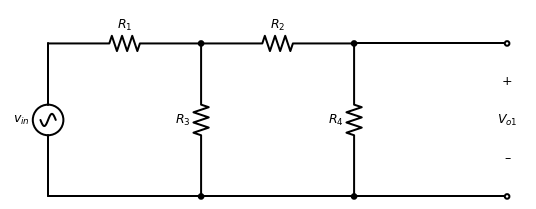
\includegraphics[scale=0.65]{p1.png}
% \caption{Original circuit schematic.}
% \label{fig:og_circ}
% \end{figure}

%%%%%%%%%%%%%%%%%%%%%%%%%%%%%%%%%%%%%%%%%%%%
%                 FIGURE                   %
%%%%%%%%%%%%%%%%%%%%%%%%%%%%%%%%%%%%%%%%%%%%
% \begin{figure}[H]
% \centering
% \begin{tabular}{cc}
% \includegraphics[width=.45\columnwidth]{step_input} &
% \includegraphics[width=.45\columnwidth]{exp_slew}\\
% (a) & (b)\\
% \end{tabular}
% \caption{(a) The input step function is applied at time $t=0\,s$.  (b) Ideally, the output would approach the input with an exponential response and time constant commensurate inversely with the bandwidth of the amplifier. In practice, if the step is sufficiently large, the amplifier experiences slew rate limiting.}
% \label{fig:step_input}
% \end{figure}

%%%%%%%%%%%%%%%%%%%%%%%%%%%%%%%%%%%%%%%%%%%%%%%%%%%%%%%%%%%%%%%%%%%%%%%%%%%%%%%%%%%%%%%%%%%%%%%%%%%%%%%%%%%
%                                           PHYSICS SYMBOLS                                               %
%%%%%%%%%%%%%%%%%%%%%%%%%%%%%%%%%%%%%%%%%%%%%%%%%%%%%%%%%%%%%%%%%%%%%%%%%%%%%%%%%%%%%%%%%%%%%%%%%%%%%%%%%%%
% \mathcal{E} % electric field
% \varepsilon % permittivity

%%%%%%%%%%%%%%%%%%%%%%%%%%%%%%%%%%%%%%%%%%%%%%%%%%%%%%%%%%%%%%%%%%%%%%%%%%%%%%%%%%%%%%%%%%%%%%%%%%%%%%%%%%%
%                                           CONSTANTS                                                     %
%%%%%%%%%%%%%%%%%%%%%%%%%%%%%%%%%%%%%%%%%%%%%%%%%%%%%%%%%%%%%%%%%%%%%%%%%%%%%%%%%%%%%%%%%%%%%%%%%%%%%%%%%%%
% Charge:
%   $\num{1.60217662e-19}C$

% Kelvin:
%   $T=300^{\circ}K$

% Permittivity in Si
%   $\epsilon_s = \num{1.03545e-10}\;F/m$
%   $\epsilon_s = \num{1.03545e-12}\;F/cm}$

%%%%%%%%%%%%%%%%%%%%%%%%%%%%%%%%%%%%%%%%%%%%%%%%%%%%%%%%%%%%%%%%%%%%%%%%%%%%%%%%%%%%%%%%%%%%%%%%%%%%%%%%%%%
%                                           EQUATIONS                                                     %
%%%%%%%%%%%%%%%%%%%%%%%%%%%%%%%%%%%%%%%%%%%%%%%%%%%%%%%%%%%%%%%%%%%%%%%%%%%%%%%%%%%%%%%%%%%%%%%%%%%%%%%%%%%
% Diffusion:
%   $\vec{J}_{n_{diff}} &= q \cdot D_N \cdot \frac{dn}{dx}$
%   $\vec{J}_{p_{diff}} &= -q \cdot D_P \cdot \frac{dp}{dx}$

% Built-in Voltage
%   $\phi_{bi} = \frac{kT}{q} \cdot ln\;\bigg( \frac{N_D \cdot N_A}{{n_i}^2} \bigg)$

% Total Depletion Region Width
%   $W_{dep} = \sqrt{\frac{2\epsilon_s \phi_{bi}}{q} \cdot \Bigg( \frac{1}{N_A} + \frac{1}{N_D} \Bigg)}$

% Individual Depletion Widths for Applied Bias
%   x_p = \sqrt{\frac{2\epsilon_s}{q} \cdot \Bigg( \frac{N_D}{N_A(N_A + N_D)} \bigg) \cdot \Bigg( \phi_{bi} - V_{applied} \bigg)}
%   x_n = \sqrt{\frac{2\epsilon_s}{q} \cdot \Bigg( \frac{N_A}{N_D(N_A + N_D)} \bigg) \cdot \Bigg( \phi_{bi} - V_{applied} \bigg)}

% Integral Forms
%   \large{y} = \int_{0}^{L} x} \,dx\
%   \[ \oint_V f(s) \,ds \]

% Maximum Electric Field
%   $\lvert \mathcal{E}_{MAX} \rvert = \lvert x_n \rvert \cdot \frac{q \cdot N_D}{\epsilon_s} = \lvert x_p \rvert \cdot \frac{q \cdot N_A}{\epsilon_s}$

% Electric Field in Terms of Potential
%   $\large{\vec{\mathcal{E}}(x)} = -\frac{dV}{dx} = -\int_{-x_p}^{x_n} \frac{\rho}{\epsilon_{si}} \,dx\$

% Poisson's Equation is defined as:
%   $\nabla \cdot \vec{\mathcal{E}} = \Large{\frac{\rho}{\epsilon}}$

% Depletion capacitance
% $C_{dep} = A \left(\frac{\epsilon_s}{W_{dep}}\right)$

% Depletion capacitance linear relationship to reverse bias
% $\frac{1}{{C_{dep}}^2} &= \frac{{W_{dep}}^2}{A^2\,{\epsilon_s}^2} = \frac{2(\phi_{bi} + V_{rev})}{q N \epsilon_s A^2}$

% NMOS saturation current
% \begin{align}
%     \Aboxed{I_{DS,sat} = \left(\frac{W}{2L}\right) \mu\,C_{ox}
%                             {\big(V_{GS} - V_{T_n}\big)}^2 (1 + \lambda V_{DS})}
%     &\textit{$PMOS$ saturation current}
%     \label{eq:mosfet_ids_nmos}
% \end{align}

% PMOS saturation current
% \begin{align}
%     \Aboxed{I_{SD,sat} = \left(\frac{W}{2L}\right) \mu\,C_{ox}
%                             {\big(V_{SG} - \left|V_{T_p}\right|\big)}^2 (1 + \lambda V_{SD})}
%     &\textit{$PMOS$ saturation current}
%     \label{eq:mosfet_ids_pmos}
% \end{align}

% NMOS triode current
% \begin{equation}
%     \boxed{I_{DS,tri} = \left(\frac{W}{L}\right) \mu_n\,C_{ox} \left(V_{GS} - V_{T_n} - \frac{V_{DS}}{2}\right) V_{DS}}
% \end{equation}

% PMOS triode current
% \begin{equation}
%     \boxed{I_{SD,tri} = \left(\frac{W}{L}\right) \mu_p\,C_{ox} \left(V_{SG} - \left|V_{T_p}\right| - \frac{V_{SD}}{2}\right) V_{SD}}
% \end{equation}

% Regions of operations
% \begin{table}[H]
% \centering
% \setlength{\tabcolsep}{20pt}
% \renewcommand{\arraystretch}{1.5}
% \begin{tabular}{|l|c|c|c|}
%     \hline
%     \textbf{Transistor Type}  &  \textbf{Cut-off} & \textbf{Triode} & \textbf{Saturation}\\
%     \hline
%     \textit{NMOS} & $V_{GS} \leq V_{T_n}$
%                     & $V_{DS} \leq V_{GS} - V_{T_n}$
%                     & $V_{DS} > V_{GS} - V_{T_n}$\\
%     \hline
%     \textit{PMOS} & $V_{SG} \leq \left|V_{T_p}\right|$
%                     & $V_{SD} \leq V_{SG} - \left|V_{T_p}\right|$
%                     & $V_{SD} > V_{SG} - \left|V_{T_p}\right|$\\
%     \hline
% \end{tabular}
% \caption{Conditions for MOSFET regions of operation.
% \label{tab:imp}} 
% \end{table}
